%==============================================================
% Part 1 : The introduction 
%==============================================================
\let\rbackup\r
\newcommand{\x}{{\mathbf{x}}}
\renewcommand{\u}{{\mathbf{u}}}
\newcommand{\w}{\mathbf{w}}
\newcommand{\y}{{\mathbf{y}}}
\newcommand{\bx}{\x}
\newcommand{\bu}{\u}
\newcommand{\bv}{v}
\newcommand{\btau}{\tau}
\newcommand{\by}{{\tilde\y}}
\newcommandx{\xb}[2][1=n,2=k]{\x_{#1|#2}}
\newcommandx{\ub}[2][1=n,2=k]{\u_{#1|#2}}
\newcommandx{\wb}[2][1=n,2=k]{\w_{#1|#2}}
\renewcommand{\r}{\mathbf{r}}
\newcommand{\rx}{\r^\x}
\newcommand{\ru}{\r^\u}
\newcommand{\vv}{{{v}}}
\newcommandx{\gb}[3][1=n,2=k,3={}]{g_{#1|#2}^{#3}}
\newcommandx{\hb}[3][1=n,2=k,3={}]{h_{#1}^{#3}}
\newcommandx{\vb}[2][1=n,2=k]{\vv_{#1|#2}}
\newcommandx{\tb}[2][1=n,2=k]{\tau_{#1|#2}}
\newcommand{\blambda}{{\boldsymbol{\lambda}}}
\newcommand{\bmu}{{\boldsymbol{\mu}}}
\newcommand{\rr}{{\mathrm{r}}}
\newcommand{\ff}{\mathrm{f}}
\newcommand{\bxi}{{\boldsymbol{\xi}}}
\newcommand{\bet}{{\boldsymbol{\nu}}}
\newcommand{\ped}{\mathrm{ped}}
\newcommand{\rped}{\r^\ped}
\newcommand{\rxped}{\r^{\x,\ped}}
\newcommand{\ruped}{\r^{\u,\ped}}

\newcommand{\matr}[2]{\left[\begin{array}{#1}#2\end{array}\right]}

\chapter{Introduction}\label{chapter:intro}
The way of transportation is in a transformation phase and autonomous driving technology is expected to have a big impact. Over one million people are killed in traffic-related accidents each year, where the vast majority of the accidents are caused by human mistakes~\cite{WHO2018, NHTSA2018}. 

Autonomous driving technology is expected to have a massive effect on the current transportation system and benefit society in many ways. For example, over one million people are killed in traffic-related accidents each year, where the vast majority of the accidents are caused by human mistakes~\cite{WHO2018, NHTSA2018}. By removing humans from the control of the vehicles, autonomous driving could significantly improve the traffic safety. Furthermore, the productivity of commercial heavy vehicles is increased when fewer human drivers are required, and the road infrastructure could be utilized more efficiently by scheduling transports outside of rush hours, for example during nights~\cite{FAGNANT2015167}.

Major progress towards deploying autonomous vehicles has been made during the last decade. The perception systems have been remarkably improved, largely due to the success of deep learning techniques~\cite{Janai2020}. The low-level control of the vehicle is a mature research area and can be solved with classical control theory methods~\cite{Paden2016}. However, how to approach the high-level decision-making in complex traffic situations is less explored and forms the main topic of this thesis.

\section{Problem formulation}
The work presented in this thesis has in particular focused on the following research questions:
\begin{enumerate}
	\item[\textbf{Q1.}] How can RL be used to create a decision-making agent for autonomous driving, that can handle different intersection and roundabouts (complex urban scenarios)? Learn a scalable policy that is able to handle different scenarios. relative coordinate system. Action space. 
	(specificera for att komma undan varfor har du inte kollat pa andra metoder. How can we use RL for AD )
	\item[\textbf{Q2.}] How can AD domain knowlage (and models) be used to improve the action and state space for a RL agent? MPC for actions, Particle filter for intention distrubution. How can AD domain knowlage be used to create a state and action space that improves the RL agent?
	\item[\textbf{Q3.}] How can the quality of a RL agent be imporved by accounting for uncertainty?
	(How can the uncertainty of the RL agent be utilized?) (RPF-in the output and PF-in the input space)
\end{enumerate}



\begin{enumerate}
	\item We want to drive through intersections. 
	\item The intersection can be of different shapes. We assume we have a map of the intersection. 
	\item There will be other cars crossing the same intersection. 
	\item We have access to sensors on-board the ego vehicle. 
	\item We dont assume any knowlage of traffic signs or traffic lights. 
	\item We dont have v2v, or v2x communication. 
	
	To compensate for not having v2v or v2x communitaion, we have to predict what other driver will do. 
	
\end{enumerate}



\section{Scope and limitations}
FILL

\section{System architecture}
outline system architecture and limit this papre to comfortable decisions \gls{rl}

\begin{figure}[t]
	\centering
	\mbox{\parbox{\textwidth}{
			\centering
			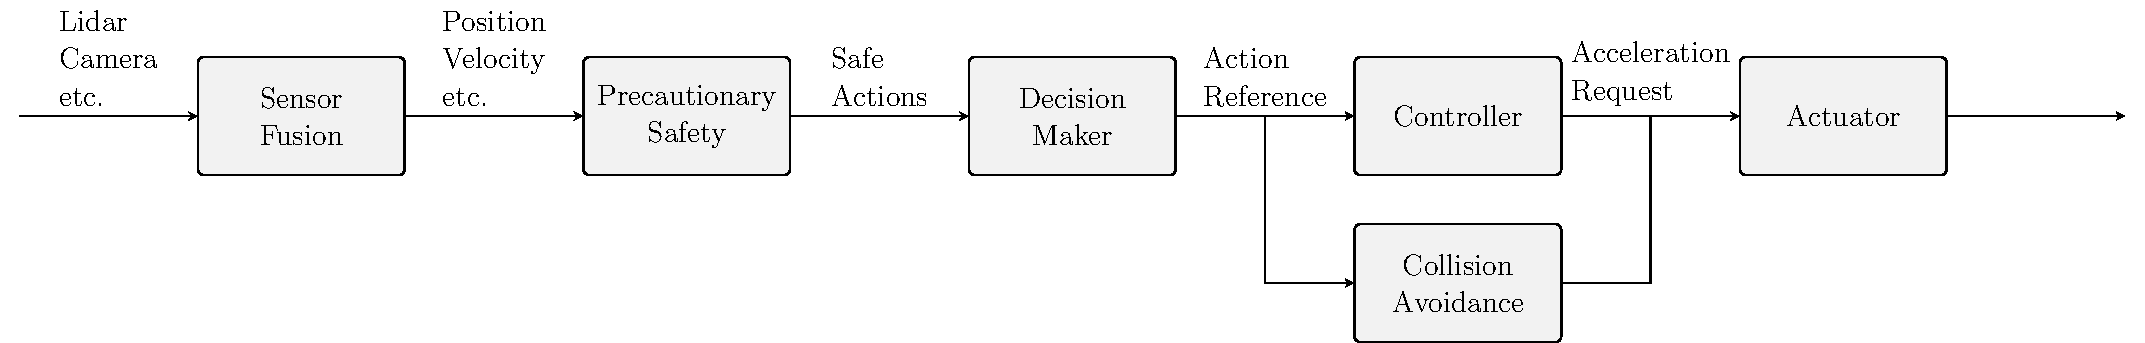
\includegraphics[width=\linewidth]{YourThesis/chapters/figures/pomdp/figures-system_architecture.pdf}%We suggest that you use a text box to insert a graphic (which is ideally a 300 dpi TIFF or EPS file, with all fonts embedded) because, in an document, this method is somewhat more stable than directly inserting a picture.   
	}}
	\caption{Representation of the system architecture.
	}
	\label{fig:system_architecture}
\end{figure}

\section{Contributions}

The main contributions of this thesis are:
\begin{enumerate}
	\item FILL

\end{enumerate}


\section{Thesis outline}
FILL



% !TEX root=../../Thesis.tex
\chapter{Related work}\label{chapter:related_work}

\todo{Urban challange, winner Carnegie Mellon University John Dolan}
\todo{Rule based methods}
\todo{Motion planning, Predicting motion of surrounding vehicles, reactive (not intersactive)}
MPC cite ivo:
A robust scenario MPC approach for uncertain multi-modal obstacles,
Real-Time Constrained Trajectory Planning and Vehicle Control for Proactive Autonomous Driving With Road Users.

\todo{POMDP model, online and offline solvers}
Cite Maxime: 
Cooperation-aware reinforcement learning for merging in dense traffic, 
Belief state planning for autonomously navigating urban intersections.
\todo{online solvers, MCTS}
MCTS cite CJ:
Combining planning and deep reinforcement learning in tactical decision making for autonomous driving,
Tactical decision-making in autonomous driving by reinforcement learning with uncertainty estimation.

\todo{cite Bo wahlberg, Morteza Haghir Chehreghani, Fernandez Llorca David, Christian Berge}

\tommy{rewrite text}
%Rule based methods
Early approaches to tactical decision-making for autonomous vehicles often used rule-based methods, commonly implemented as handcrafted state machines. For example, during the DARPA Urban Challenge, a rule-based approach was adopted by the winning team from the Carnegie Mellon University, where different modules handled the behavior for the different driving scenarios that were encountered~\cite{darpaCMU}. Other participants, such as Stanford and Virginia Tech, used similar strategies~\cite{Bacha2008, darpaStanford}. While successful for a limited and controlled environment such as the Urban Challenge event, it is unlikely that rule-based approaches could scale to handle the complexity and diversity of real-world driving.

%Motion planning, predicting motion of surrounding vehicles, reactive (not interactive)
Another group of algorithms treats the decision-making task as a motion planning problem. Commonly, a prediction model is used to predict the motion of the other agents, and then the behavior of the vehicle that is being controlled, henceforth referred to as the ego vehicle, is planned accordingly. This results in a reactive behavior, since the predictions are independent of the ego vehicle plan. Therefore, interaction between the ego vehicle and other agents is not explicitly considered, but may happen implicitly by frequent replanning.
Search-based planners typically discretize the state space and then apply Dijkstra's algorithm~\cite{Dijkstra1959} or one of the algorithms from the A* family~\cite{Hart1968}. These techniques were also commonly used during the DARPA Urban Challenge~\cite{Bacha2008, darpaStanford}. However, since real-time performance can be hard to achieve with graph-search algorithms, sampling-based algorithms such as rapidly-exploring random trees~\cite{Lavalle1998} have been used for motion planning, e.g., by Karaman et al.~\cite{Karaman2011}. A third approach to solve the motion planning problem is to use optimization-based techniques, for example optimal control, which was applied to highway driving scenarios by Werling et al.~\cite{Werling2010}. Since human behavior is complex and varies between individuals, some algorithms use a probabilistic prediction as input to the motion planning. This is for example shown in a study by Damerow et al.~\cite{Damerow2015}, which aims to minimize the risk during an intersection scenario.
Additional approaches to motion planning for autonomous driving are provided in the surveys by Gonzáles et al.~\cite{Gonzales2016} and Paden et al.~\cite{Paden2016}. 


%POMDP model, online and offline solvers
It is common to model decision-making problems as Markov decision processes or partially observable Markov decision processes (POMDPs)~\cite{Kochenderfer2015}. This mathematical framework allows modeling of uncertainty in the current state, uncertainty in the future development of the traffic scene, and modeling of an interactive behavior. The task of finding the optimal policy for a POMDP is most often intractable, but many approximate methods exist. One way to group these methods is in offline and online methods. There are powerful offline algorithms for planning in POMDPs, which can solve complex situations. One example is shown by Brechtel et al., which proposes a solution to how measurement uncertainty and occlusions in an intersection can be handled~\cite{Brechtel2014}. In their work, an offline planner precomputes the policy by using a state representation that is learned for the specific scenario. A similar approach is adopted by Bai et al.\ for an intersection scenario~\cite{Bai2014}. The main drawback of these offline methods is that they are designed for specific scenarios. Due to the large number of possible real-world scenarios, it is challenging to precalculate a policy that is generally valid.


%Online solvers
Online methods compute a policy during execution, which makes them more versatile than offline methods. However, the limited available computational resources require a careful problem formulation and limit the solution quality.
Ulbrich et al.\ use a POMDP framework to make decisions on when to change lanes during highway driving~\cite{Ulbrich2015}. In order to make it possible to solve the problem with an exhaustive search, a problem-specific high-level state space is created, which consists of states that represent whether or not a lane change is possible or beneficial. However, due to the specialized state space, it is hard to generalize this method.
Another online approach for solving a POMDP is the family of Monte Carlo tree search algorithms~\cite{Browne2012}, which is used by Sunberg et al.\ to make lane changing decisions on a highway~\cite{Sunberg2017}. In order to handle the continuous state description, the tree search is extended with a technique called progressive widening~\cite{Couetoux2011}. Furthermore, other drivers' intentions are estimated with a particle filter. %\cite{Lenz2016} also applied a MCTS method for lane change decisions.
A hybrid approach between offline and online planning is pursued in a study by Sonu et al., where a hierarchical decision-making structure is used~\cite{Sonu2018}. The decision-making problem is modeled on two levels as MDPs, since full observability is assumed. The high-level MDP is solved offline by value iteration and the low-level MDP is solved online with MCTS.
% Requires transition model, hard to obtain.


\vspace{8pt}

\section{Learning-based methods}

In planning-based methods, different algorithms are used to find a policy that maximizes the utility of the agent's behavior by using a model of the system. However, data-driven approaches are fundamentally different, since with this class of methods, an agent instead learns how to behave from observing data. This section describes different types of data-driven approaches that have been explored for autonomous driving.

% Imitation learning, behavioral cloning
An intuitive approach is to collect data from when an expert is performing a task and then use supervised learning to imitate the behavior of the expert. This method is often referred to as behavioral cloning and was first applied to autonomous driving in the ALVINN project~\cite{Pomerleau1989}. Unfortunately, for many cases, behavioral cloning suffers from compounding errors, which refers to the problem when small mistakes gradually push the agent further away from the training distribution, into states from which the agent does not know how to recover. This problem can be mitigated by an active learning approach, where an expert can be queried during the training process~\cite{Ross2011}, which for example has been applied to autonomous driving by Kelly et al.~\cite{Kelly2019}. An alternative is to synthesize data by perturbing the expert's driving, which was done in a study by Bansal et al.~\cite{Bansal2019}. Generative adversarial imitation learning~\cite{Ho2016} provides another method to handle the compounding error problem and has showed promising results in different highway driving scenarios~\cite{Kuefler2017}.

%RL
Reinforcement learning is conceptually different from supervised learning, since labeled input-output samples are not available. Instead, the agent learns how to make decisions from interacting with the environment.
%Reinforcement learning is conceptually different from supervised learning, which is used for behavioral cloning, since labeled input/output samples are not available in RL problems. Instead, an RL-based agent typically learns how to make decisions from interacting with an environment, in which the agent occasionally receives a reward signal that tells the agent how well it is performing.
RL methods are versatile, and have proven successful in various domains, such as playing Atari games~\cite{Mnih2015}, in continuous control~\cite{Lillicrap2015}, reaching a super human performance in the game of Go~\cite{Silver2017}, and beating the best chess computers~\cite{Silver2017chess}. One advantage of RL methods, compared to planning based methods, is that a model of the environment is not required, i.e., the transition probabilities between different states are not assumed to be known. Furthermore, many RL methods provide a general framework and an agent could, in theory, learn how to behave correctly in all possible driving situations.
%
During the last few years, many papers have addressed the task of applying RL approaches to autonomous driving. For example, DQN-based agents were used by Tram et al.~\cite{Tram2018} and Isele et al.~\cite{Isele2018} for navigating through different intersection scenarios, with varying driver intentions and occlusions. Commonly, a high-level action space is used together with the DQN algorithm. Other studies use policy gradient RL methods to directly control the speed and the steering angle of the vehicle, for example in lane changing and urban scenarios~\cite{Wang2019_ddpg, Chen2019}.
Safety of the RL-based agents has been addressed by restricting dangerous actions, either by heuristics~\cite{Mukadam2017}, linear temporal logic~\cite{Bouton2019}, or using an underlying motion planner with hard constraints~\cite{Shalev2016}.
%
%A Deep Q-Network agent that can learn how to negotiate an intersection, while interacting with drivers with different intentions, is presented by Tram et al.~\cite{Tram2018}. This approach uses a high level state description and action space.
%In a previous paper, we showed how a Deep Q-Network (DQN) agent could learn when to change lanes and how to control its speed in a one-way highway scenario and in a two way overtaking scenario, using a high level state input~\cite{Paper2}. A novel neural network architecture, that simplifies the handling of multiple agents, was also introduced. A similar approach, using a DQN, was presented by Tram et al., but applied to an intersection scenario~\cite{Tram2018}.
%A DQN agent is also used by Isele et al., who consider several different intersection scenarios, but uses a discretized bird's eye view description of the state, which can also represent occluded areas~\cite{Isele2018}. Expert knowledge that restrict certain actions can be utilized, which can speed up the training process for a lane changing scenario~\cite{Mukadam2017}. A different approach is presented by Shalev et al., applied to a merging scenario on a highway, where a policy gradient method is used to learn a desired behavior. At every time step, the desires are then mapped to an actual trajectory by solving an optimization problem with hard constraints, which guarantees safety~\cite{Shalev2016}.
A majority of these studies perform both the training and evaluation in simulated environments, whereas some train the agent in a simulator and then apply the trained agent in the real world~\cite{Pan2017, Bansal2019}, or for some limited scenarios, the training itself is also performed in the real world~\cite{Kendall2019}. 
Overviews of RL-based studies for autonomous driving are given by Kiran et al.~\cite{Kiran2021} and by Ye et al.~\cite{Ye2021}.
% Add reference to Pin Wang's new review paper. Possibly replace one of the other survey papers?
%    - DONE

Both planning-based and RL-based methods use a reward function to find a policy that maximizes the cumulative future reward. However, for complex tasks such as autonomous driving, the design of the reward function is in itself a complicated task. For limited scenarios, the reward function can be manually specified and tuned until the agent finds a desired behavior, which is referred to as reward shaping~\cite{Ng1999}. However, for realistic scenarios, the number of possible reward features is massive and how to balance rewards related to, e.g., safety and efficiency is a complex issue. A practical approach is to instead learn the reward function from the behavior of human drivers by inverse reinforcement learning (IRL)~\cite{Ng2000}. An IRL approach was for example used by Kuderer et al.\ to learn the individual preferences of human drivers with different driving styles~\cite{Kuderer2015}. Sharifzadeh et al.\ combined IRL with DQN and Wang et al.\ used an adversarial IRL approach to simultaneously obtain both the reward function and the policy for different lane-changing scenarios~\cite{Sharifzadeh2016, Wang2019}. 
Zhu et al.~\cite{Zhu2021} provide an overview of IRL applied to autonomous driving.
Except for performing planning and RL, the learned reward function can also be used to predict the behavior of other traffic participants. IRL for predictions was for example used by Ziebart et al.\ for pedestrians~\cite{Ziebart2009}, by Sun et al.\ for human drivers in intersections~\cite{Sun2019}, and by Sadigh for highway driving situations~\cite{Sadigh2016}.


% !TEX root=../../Thesis.tex
\chapter{Technical Background}\label{chapter:background}
%

\section{Partially Observable Markov Decision Process}\label{section:pomdp}

\begin{itemize}
    \item POMDP
    \item State - realative features, scalable to fidderent types of intersection design 
    \item Action - IDM - MPC
    \item Observation - unknown intentions, red lights, stop signs yield. 
    \item Transistion function - RL 
    \item Reward Function - Goal, Comfort, crash
    \item discount factor 
\end{itemize}

\chapter{Technical background}
\label{ch:theoreticalBackground}

% Now not using time index, e.g., s_t. Check if consistent with subsequent chapters.
%    - Time index not used (much) in Paper 2-5, but in Paper 6. Slighlty inconsistent at the moment, but doesn't matter too much...

% This chapter gives a brief introduction to
% %how the problem of making sequential decisions based on uncertain information can be modeled, 
% Markov decisions processes
% and reinforcement learning. Notation that is used in subsequent chapters is also introduced. The material in this chapter is based on Kochenderfer~\cite{Kochenderfer2015} and Sutton et al.~\cite{Sutton2018}, which provide a comprehensive overview of MDPs and RL.

This chapter provides a brief introduction to Markov decision processes and reinforcement learning.
%, together with the notation that is used in subsequent chapters. 
% The reader who is familiar with these concepts could probably skip this chapter and return in case of any confusion concerning the notation. 
The purpose of the chapter is to summarize the most important concepts and introduce the notation that are used in the subsequent chapters. 
A comprehensive overview of MDPs and RL is given in the books by Kochenderfer~\cite{Kochenderfer2015} and Sutton and Barto~\cite{Sutton2018}, upon which this chapter is based.


\section{Markov decision processes}
\label{sec:mdp}
%MDP
Sequential decision-making problems in stochastic environments are commonly modeled as MDPs. Importantly, an MDP satisfies the Markov property, which requires that the probability distribution of the next state only depends on the current state and the action taken by the agent, i.e., not on the history of previous states or actions. An MDP is formally defined as the tuple $( \mathcal{S}, \mathcal{A}, T, R, \gamma )$, which is described in the following list~\cite[Ch. 4]{Kochenderfer2015}:
%
\begin{itemize}
    \item The state space $\mathcal{S}$ represents the set of all possible states of the environment. This set could consist of both discrete and continuous states.
    \item The action space $\mathcal{A}$ represents the set of all valid actions the agent can take. This set could also consist of both discrete and continuous actions. However, since this thesis focuses on high-level decision-making, only discrete actions are considered here.
    \item The state transition model $T(s'|s,a)$ describes the probability that the system transitions to state $s' \in \mathcal{S}$ from state $s \in \mathcal{S}$ when action $a \in \mathcal{A}$ is taken.
    \item The reward function $R(s,a)$ returns a scalar reward $r$ for each state-action pair.
    \item The discount factor $\gamma \in [0,1)$ is a scalar that discounts the value of future rewards. For a finite horizon MDP, $\gamma$ could also take the value~$1$.
\end{itemize}

A policy $\pi$ is a mapping from a state to an action, which could either be deterministic $a=\pi(s)$ or probabilistic $a \sim \pi(a|s)$. The value of being in a state while following a policy is described by the value function
%
\begin{align}
    V^\pi(s) = \mathbb{E} \left[ \sum_{k=0}^\infty \gamma^k R(s_k, a_k) | s_0 = s, \pi \right].
\end{align}
%
The goal of the agent is to find a policy which maximizes the value of each state.

% In this framework, an agent chooses an action $a$, based on the current state $s$, then receives a reward $r$, and transitions to a new state $s'$. An MDP satisfies the Markov property, which assumes that the probability distribution of the next state only depends on the current state and action, and not on the history of previous states. The MDP is defined as the tuple $( \mathcal{S}, \mathcal{A}, T, R, \gamma )$, where $\mathcal{S}$ is the state space, $\mathcal{A}$ is the action space, $T$ is a state transition model, $R$ is a reward model, and $\gamma \in [0,1]$ is a discount factor. 
% The state transition model $T(s' \mid s,a)$ describes the probability that the system transitions to state $s'$ from state $s$ when action $a$ is taken, and the reward model defines the reward of each step as $r=R(s,a,s')$.
% The goal of an agent is to find a policy $\pi(s)$ which for every time step $t$ chooses an action that maximizes the future discounted return $R_t$, defined as
% %
% \begin{align}
%     \label{eq:discountedReturn}
%     R_t = \sum_{k=0}^\infty \gamma^k r_{t+k},
% \end{align}
% %
% where $r_{t+k}$ is the reward at step $t+k$.


%POMDP
In many decision-making problems, the agent does not have direct access to the state of the environment. Such a problem is commonly modeled as a partially observable Markov decision process, which is an extension to the MDP framework that also models state uncertainty. A POMDP is formally defined as the tuple  $( \mathcal{S}, \mathcal{A}, \mathcal{O}, T, O, R, \gamma )$, where the state space, action space, transition model, reward function, and discount factor are defined as for an MDP. A POMDP has two additional components~\cite[Ch. 6]{Kochenderfer2015}:
%
\begin{itemize}
    \item The observation space $\mathcal{O}$, which is the set of possible observations.
    \item The observation model $O(o|s',a)$, which describes the probability of observing $o \in \mathcal{O}$ in state $s'$ after action $a$ has been taken.
\end{itemize}
%
Since the agent does not have direct access to the current state in a POMDP, the agent needs to reason about the history of observations and actions. This history is often merged in a belief state $b$, which represents a probability distribution over the state space. In this case, the policy is a mapping from beliefs to actions $\pi(b)$.



%In many decision-making problems, the exact state is not known by the agent and it only perceives observations $o$. A problem with state uncertainty can be modeled as a partially observable Markov decision process, which is defined by the tuple $( \mathcal{S}, \mathcal{A}, \mathcal{O}, T, O, R, \gamma )$. Compared to an MDP, the POMDP includes an additional observation space $\mathcal{O}$, and an observation model $O(o \mid s,a,s')$, which describes the probability of observing $o$ in state $s'$, after taking action $a$ in state $s$.


For many real-world problems, it is not possible to represent the probability distributions $T$ or $O$ explicitly. For some solution approaches, only samples are needed, and then it is sufficient to define a generative model $G$ that samples a new state or observation from a given state and action, i.e., $s' \sim G(s,a)$ for the MDP case~\cite[Ch. 4]{Kochenderfer2015} and $(s', o) \sim G(s,a)$ for the POMDP case~\cite[Ch. 6]{Kochenderfer2015}.


\section{Reinforcement learning}
\label{sec:rl}

If all the elements $( \mathcal{S}, \mathcal{A}, T, R, \gamma )$ of an MDP are known, an agent can use this model to directly compute an optimal policy. Such a problem is often considered a planning problem. For small MDPs, dynamic programming\footnote{Dynamic programming refers to simplifying a complex problem by breaking it down into smaller sub-problems, often in a recursive manner.} techniques can provide an exact solution, which is calculated offline, i.e., before the agent is deployed in the environment. For example, in value iteration~\cite[Ch. 4]{Kochenderfer2015}, the Bellman operator is iteratively applied to the value function for all states,
%
\begin{align}
    V_{n+1}(s) = \max_a \left[ R(s,a) + \gamma \sum_{s'}T(s'|,a,s)V_n(s') \right].
\end{align}
%
As $n$ goes to infinity, $V_n$ converges to the unique optimal value function $V^*$, and an optimal policy (not necessarily unique) is extracted by
%
\begin{align}
    \pi(s) = \argmax_a \left[ R(s,a) + \gamma \sum_{s'}T(s'|,a,s)V^*(s') \right].
\end{align}
%
However, for many real-world problems with high dimensional state spaces, it is intractable to compute and store a policy offline. Contrarily to offline methods, online search methods perform planning from the current state up to some horizon, when the agent has been deployed. Thereby, the agent can limit the computation to states that are reachable from the current state, which is often significantly smaller than the full state space~\cite[Ch. 4]{Kochenderfer2015}.

% \begin{figure}[!bt]
%     \centering
%         \vspace{-10pt} % To avoid widow word.
%         \includegraphics[width=0.7\columnwidth]{figures/RL_cropped.pdf}
%         \caption{In a reinforcement learning problem, an agent learns a policy $\pi$ by interacting with its environment. The agent collects experience by repeatedly taking actions and then observing the resulting state and reward.}
%         \vspace{-10pt} % To avoid widow word.
%     \label{fig:RL}
% \end{figure}

In many problems, the state transition probabilities or the reward function are not known. These problems can be solved by reinforcement learning techniques, in which the agent learns how to behave from interacting with the environment~\cite[Ch. 5]{Kochenderfer2015}, see Figure~\ref{fig:RL}. Compared to supervised learning, reinforcement learning presents some additional challenges. Since the data that are available to an RL-agent depends on its current policy, the agent must balance exploring the environment and exploiting the knowledge it has already gained. Furthermore, a reward that the agent receives may depend on a crucial decision that was taken earlier in time, which makes it important to assign rewards to the correct decisions.

%If MDP is known, planning. RL deals with unknown T or G, interacts with environment to learn. Figure.
% As mentioned above, the goal of a decision-making agent is to take actions that maximizes the future discounted return $R_t$. If all elements of the MDP are known, the agent could compute which action that is ideal before executing any actions in the environment, which is referred to as planning. However, in many problems the transition model or generative model is not known to the agent beforehand and it needs to learn how to behave from experience, which is referred to as a reinforcement learning problem. The agent will then act in the environment and observe what happens, in order to figure out a policy $\pi$, which defines which action to take in a given state.
% Figure~\ref{fig:RL} shows a schematic overview of the reinforcement learning problem.
% The agent is commonly represented by a neural network, which acts as a nonlinear function approximator. Further details on neural networks and how they can be used in RL are described by Sutton et al.~\cite{Sutton2018}.


%Reinforcement learning is a class of machine learning techniques, which enables an agent to learn a policy $\pi$ that maximizes the expected future return $\mathbb{E}(R_t)$ in the environment the agent acts in~\cite{Sutton1998}. 



%Model based vs model-free
% Model based - learns model T, then planning
% Model free - does not learn model
% Model free techniques range from direct policy search vs value-based RL

%One approach to decide which action to take is to first try to learn the model of the environment from the observations, i.e., to learn $T$. Once the model is learned, a planning algorithm could be used to find the best policy. RL approaches that follows this structure are called model based RL algorithms.

RL algorithms can be divided into model-based and model-free approaches~\cite[Ch. 5]{Kochenderfer2015}. In the model-based versions, the agent first tries to estimate a representation of the state transition function $T$ and then use a planning algorithm to find a policy. On the contrary, as the name suggests, model-free RL algorithms do not explicitly construct a model of the environment to decide which actions to take. 
The model-free approaches can be further divided into value-based and policy-based techniques. Value-based algorithms, such as $Q$-learning, aim to learn the value of each state and thereby implicitly define a policy. Policy-based techniques instead search for the optimal policy directly in the policy space, either by policy gradient methods or gradient-free methods, such as evolutionary optimization. There are also hybrid techniques that are both policy and value-based, such as actor critic methods.


% Genetic algorithms belong to a family of optimization methods that are inspired by the evolutionary mechanisms of natural selection~\cite{Holland1975}.
% In general, GAs are suitable for solving optimization problems where the objective function is non-differentiable, or even when an explicit mathematical model does not exist and only a simulation is available. 
% A GA can also solve some versions of RL problems, and is used as an RL method in this thesis.


RL algorithms generally assume that the environment is modeled as an MDP, i.e., that the state of the environment is known by the agent. However, in many cases of interest, only partial information about the state of the environment is available, which is modeled in the POMDP framework. For such cases, it is common to approximate the state by either the observation or a finite history of observations~\cite[Ch. 17]{Sutton2018}. The latter is referred to as a $k$-Markov approximation, where $k$ defines the length of the included history. For a sufficiently long history, the Markov property is assumed to approximately hold, even though the environment is partially observable.

% Possibly add something about neural networks as function approximators somewhere in this section?
%    - No

% !TEX root=../../Thesis.tex
\chapter{Model-free RL approaches}
\section{State representation}
This section describe the general state representation used in this research that enables these methods to be generalizable for different type of intersection and crossings. 
By describing the state space as a set of distances to intersection points, we can abstract the map layout of different intersections and the same algorithms would work for intersections variations that we havent specifically trained on. 
\todo{add image of intersection scenario with 90 degree entry point and 45 degree entry point.}
\subsection{Observable states}
position, velocity and acceleration. 
\subsection{Unobservable states}
intentions. traffic lights and traffic signs. 
\section{Approach}
\section{Simulated experiments}
\section{Results and discussion}

\chapter{Combining MCP and RL}
\section{Action space, options}
\section{MPC}
\section{Approach}
MPC has a mixed integer problem, calculating the optimal path for all possible action is very computationally heavy. 
RL DQN. Only has descret actions. can not garantee safety. but is good at choosing actions with the best utility (value). 
The reward function takes in the predicted outcome of the model in the MPC and can penalize the choice of action. but if experience show that the outcome is better than the model, it can choose to take a bad action that would lead to a better total reward compared to only following a conservative model. 

\section{Simulated experiments}
We show the difference in a multi crossing scenario where the MPC can plan a path for both intersections while our previous DQN only handles one at a time. 

\section{Results and discussion}

\chapter{Estimating the uncertainty}
\todo{rewrite chapter name}

\section{Uncertainty of the decision}
\subsection{Approach}
\subsection{Simulated experiments}
\subsection{Results and discussion}

\section{Uncertrainty of the intention}
\subsection{Approach}
\subsection{Simulated experiments}
\subsection{Results and discussion}


\chapter{Generalize over different scenarios}
\section{Approach}
\section{Simulated experiments}
\section{Results and discussion}
FILL
\chapter{Discussion}
\label{ch:discussion}
Chapter 4, 5 and 6 introduce different methods to create a decision-making agent for navigating through intersections using deep Q-learning, while considering the uncertainty of its own decisions and the prediction of the other drivers intentions. This chapter highlights some differences and synergies of the different methods. 

\section{Guaranteeing safety}
\label{ch:system_architecture}
Safety is the most important factor of a \gls{ad} system, but since \gls{rl} is a data driven approach it is very difficult to guarantee safety in the same way e.g., a \gls{mpc} can. Safety validation in a data driven approach can be very costly as it is usually done by driving many miles and showing statistical confidence in the safety metrics~\cite{koopman2016,asljung2017}, e.g., number of interventions. That is why this section will clarify where the work in this thesis would fit in by first defining a system architecture for \gls{ad}, its modules and a short summary of the ISO 26262 standard. Then, place itself within the system and motivate how safety can be guarantied. 

The architecture of an autonomous driving system can be divided into perception, planning and control~\cite{Schwarting2018,Kortenkamp2008}.
The perception module is responsible for sensing and mapping the environment with the use of sensors such as LIDARs, cameras, radars etc. The raw data from the sensors are then processed though various sensor fusion techniques to generate a representation of the environment, e.g., position, velocity of other traffic participants while also describing the road such as width and distance to the next intersection. This information is then used by the planner to create a driving strategy of how to transverse through the world. However, the information from the sensors are often noisy, with false positives and false negatives making it difficult for the planner.

Tactical planning can be divided into three categories, the proactive, active and reactive~\cite{Berntorp2018}. A proactive module would be something like a precautionary safety module that interprets the information about the environment and create constraints that is sent to the active planner, like  driveable area, allowed speeds and actions~\cite{Shiller2007}. These constraints are generated from a set of safety goals and rules, making this the first layer of protection that can ensure safety. 
The role of the active planner is to take this sets of allowed actions and prescribe the behavior of the vehicle through decisions such as drive, yield or stop. The goal of these high level decisions is to optimize metrics such as comfort, fuel consumption and time to goal. These decisions are then sent to a motion planner that generates a safe dynamically feasible path for the vehicle for a shorter planning horizon of around $0.1$s. 
At the same time, a reactive, collision avoidance, module make sure that the chosen decision and path does lead to any collisions~\cite{brannstorm2010}. Unlike the decision maker, the collision avoidance module main goal is to identify imminent danger~\cite{brannstorm2014} and therefore has access to more aggressive actions like emergency braking to ensure safety. 
 
In the industry today the main standard for functional safety in motorized vehicles is the ISO 26262 standard, titled "Road vehicles – Functional safety"~\cite{ISO26262}. It uses a \gls{asil} to classify the inherent safety risk in an automotive system and the functions or modules of such a system. The \gls{asil} classification is used to express the level of risk reduction required to prevent a specific hazard, from \gls{asil} D to \gls{asil} A. \gls{asil} D represents the highest hazard level and \gls{asil} A the lowest. There is a level with no safety relevance and only standard Quality Management processes are required, this level is referred to as QM.

\begin{figure}[h]
	\centering
	%  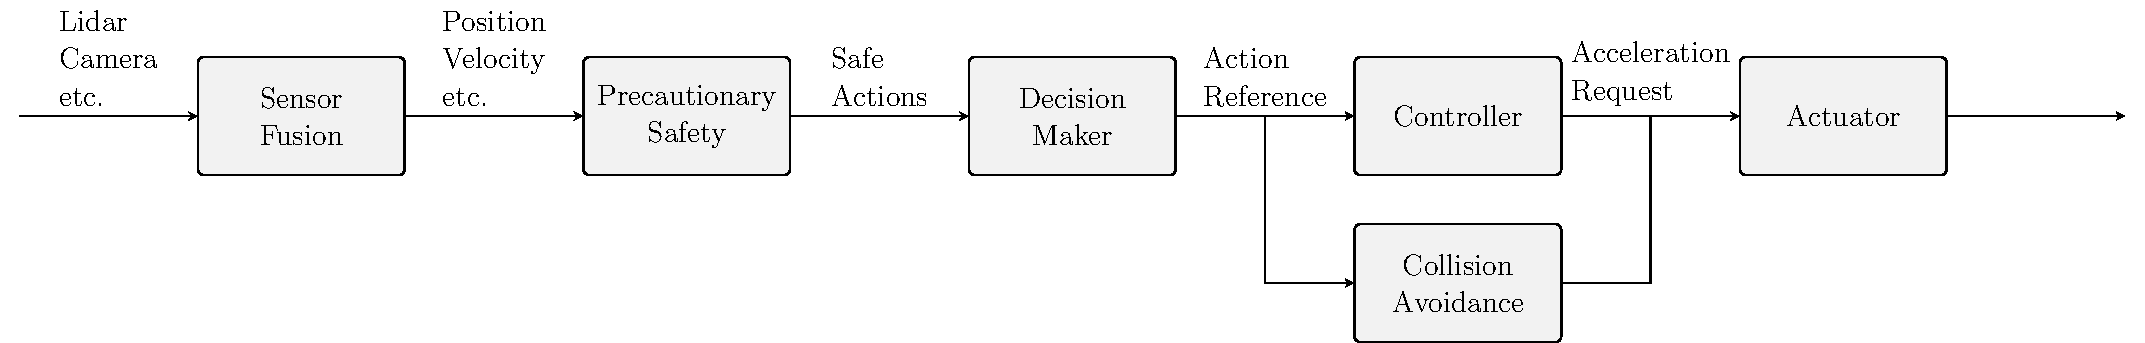
\includegraphics[width=\linewidth]{YourThesis/chapters/figures/pomdp/figures-system_architecture.pdf}
	\begin{tikzpicture}[
		node distance=8mm and 16mm,
		node font= \small,
		box/.style = {draw, thick, rectangle, rounded corners=0.1cm, fill=gray!10, minimum width=1.5cm, minimum height=1cm, align=center},
		% sx+/.style = {xshift = 1mm},
		sx+/.style = {xshift = 1mm}
		]
		
		\node (start1) at (0,0) {};
		\node[circle, draw, dashed, thick, fill=gray!30, minimum size=1.0cm] (world) {World};
		\node (SF) [box, right=of world.east] {Sensor \\ Fusion};
		\node (PS) [box, right=of SF.east] {Precautionary \\ Safety};
		\node (DM) [box, below=of PS.south] {Decision \\ Maker};
		\node (Con) [box, below=of SF] {Controller};
		\node (CA) [box, below=of Con] {Collision \\ Avoidance};
		\node (Act) [box, below=of world, yshift=.08cm] {Vehicle};
		\node (end) [left=of Act] {};

		\draw[->,thick,align=left] (world) --+(SF) node [midway,above] {Lidar\\Camera\\etc.};
		\draw[->,thick,align=left] (SF) --+(PS) node [midway,above] {Position\\Velocity\\etc.};
		\draw[->,thick,align=right] (PS) -| ($(PS.east) + (.5,0mm)$) |- (DM) node [above, xshift=10mm, yshift=5mm] {Safe\\Actions};
		\draw[->,thick,align=left] (Con) --+(Act) node [midway,above, xshift=3mm] {Acceleration\\Request};
		\draw[->,thick,align=left] (Act) -| ($(Act.west) - (.5,0mm)$) |- (world) node [midway,left] {};
		\draw[->,thick,align=left] (DM) --+(Con) node [midway,above] {Action\\Reference};
		\draw[->,thick,align=left] (DM) -| ($(DM.west) - (1,0mm)$) |- (CA) node [midway,above] {};
		\draw[->,thick,align=left] (CA) -| ($(CA.west) - (.7,0mm)$) |- (Act) node [midway,above] {};

	\end{tikzpicture} 
	\caption{Representation of the system architecture.}
	\label{fig:system_architecture}
\end{figure}

Although safety is the most important requirement for enabling autonomous driving, the work in this paper does not make any safety guarantees. Instead, it is proposed that the decision-making algorithms presented in this paper be used in the system architecture shown in Figure~\ref{fig:system_architecture}. This approach allows higher \gls{asil} to be applied to the precautionary safety and collision avoidance modules, while the decision-making algorithms focus primarily on comfort. As a result, the \gls{asil} classification for the decision-making components could be at lower levels, potentially even classified as QM in the best case.

\section{Designing the reward function and terminal states}
The reward function introduced in Chapter~\ref{ch:reward_function_def} is a crucial component that significantly influences the behavior and performance of a reinforcement learning agent. By carefully designing and tweaking the reward function in \eqref{eq:thesis_reward_function}, the agent can be guided towards desirable behaviors and optimize its decision-making policy. 

The results from Chapter~\ref*{ch:modeling_intersection} and \ref{ch:uncertainty} show a collision rate of $1-3\%$, which may seem high for \glspl{av}. However, within the proposed system architecture from Figure~\ref{fig:system_architecture}, this collision rate can be interpreted as interventions by a collision avoidance system, such as emergency braking. This interpretation can be achieved by adjusting the simulation parameters, for example, increasing the size of the cars or redefining the collision state to represent a collision avoidance intervention state.

% In comparison to \paperLSTM \ and \paperMPC, the need for a terminal state was removed for \paperEnsamble \ and \paperBelief, by excluding that state transaction in the experience replay, effectively allowing the agent to continue forever. While in \paperLSTM \ there was a negative reward for choosing an action to follow a non-existing car. This could also be removed by using Q-masking in \paperMPC \ and \paperEnsamble. 


\section{Modular models in autonomous vehicles}
There are two common strategies for creating and deploying \glspl{dqn} to the real world: training a comprehensive model that encapsulates everything or training smaller, specialized models and switching between them as needed. The proposed MLEMTRL algorithm from Chapter~\ref{ch:generalize} is a step towards the latter approach of using smaller models. Combined with the uncertainty measurements in Chapter~\ref{ch:uncertainty}, instead of reverting to a default action when uncertainty is high, the agent can instead trigger a model change. MLEMTRL can then be used to determine which model to switch to, ensuring a more adaptive and robust decision-making process.

This approach allows for modularity and flexibility, enabling easier updates and maintenance since individual models can be refined or replaced without affecting the entire system. Additionally, smaller models are less likely to overfit to irrelevant details present in a larger, comprehensive dataset, leading to more generalizable and robust performance in their specific domains. They also require less computational power and memory, making them more suitable for deployment on \gls{av}s with limited resources. Smaller models are generally easier to interpret and debug, facilitating understanding of the decision-making process and identifying any issues or biases, which is an important property to have when developing \gls{av}s.

% \section{Simulation and real world}
% Bridging the gap between simulation and real world. Ever evolving driving styles. Building trust. 
% Public trust is essential for the widespread adoption of AVs. Building this trust requires addressing concerns about safety, reliability, and the overall impact of AVs on society.
% Transparency and Communication: Providing clear and transparent information about how AV systems work, their safety features, and their limitations can help in building public trust. This includes communicating the results of safety tests and real-world performance data.
% Regulatory Compliance: Ensuring that AVs meet or exceed regulatory standards for safety and performance is crucial. Collaborating with regulatory bodies to establish and adhere to stringent safety protocols can reassure the public.
% Demonstrations and Pilot Programs: Conducting public demonstrations and pilot programs can help in showcasing the capabilities and safety of AVs. Allowing people to experience AVs firsthand can alleviate fears and misconceptions.
% !TEX root=../../Thesis.tex
\chapter{Concluding remarks and future work}
\section{Conclusions}\label{sec:conclusion}

1. RL by itself still has a long way to guarantee safety, but the methods presented in this paper. the unncertainty can be reduced. safety is better suited for contrl or formal methods. RL is a great tool for creating policy that can adapt to different driver interntions. 
2. Even with todays advancements in \gls{nn} DQN still has a hard time handling 
\section{Future work}
FILL

\includepapersummary % Label: 'chap:papersummary'. Replace with separate file if the auto-generated summary does not work with your content.

%==============================================================